
\subsubsection{Alternatives to Distributed machine learning}
Even though the most popular solution to increasing computation power for Machine
learning is currently distributing the workload over a large amount of machines
there are other more traditional ways to increase computation power. These ways
being the use of Application Specific Integrated Circuits, and special multi core
computer architectures.

\paragraph{Asics}
The idea of creating ASICs for use in highly specialized tasks is not a new idea
to machine learning, in recent times the demand for such chips has risen masively\cite{Metz18}
looking at applications such as bitcoin mining asics have had a massive competitive
advantage over GPUS and CPUS rendering them essentially useless. The main reason
that ASICs have such a good outlook when looking at machine
learning is the fact that most of the work in most areas are matrix multiplications.
This means that it is viable to have a chip that can only multiply matrixes and nothing
else.

Google took this idea of ASICs and have created their Tensor Processing Unit (TPU)\cite{Sato17}
which as the name hints is an ASIC computer that specializes in calculations that
use tensors, this works well together with their Tensor flow library which is one
of the most popular Neural Network Libraries around at the moment. Architecture of
the chip can be seen in figure \ref{TPU_Architecture}.

\begin{figure}
  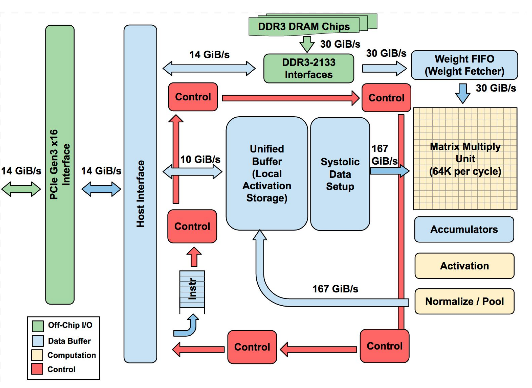
\includegraphics[width=\textwidth]{TPU_Architecture.png}
  \caption{Google TPU Architecture\cite{Joup17}}
  \label{TPU_Architecture}
\end{figure}

The most important aspect of the TPU is the Matrix Multiply unit that is positioned
on the right of the diagram. As can be seen the TPU uses a PCIe bus to communicate
with a server, so it is not a stand alone unit. Which is usefull as it can then also
be used in a distributed setting.

The performance improvement of the TPU vs a regular CPU/GPU combinations is not only
in the increased processing power, but also in the efficiency, which is important
for big companies that want to run many TPUs in the same building. In figure \ref{TPU_Relative_Performance}
it can be seen that the performance/watt relative to GPUs and CPUs of a TPU is many times higher,
up to nearly 200x the performance/watt.

\begin{figure}
  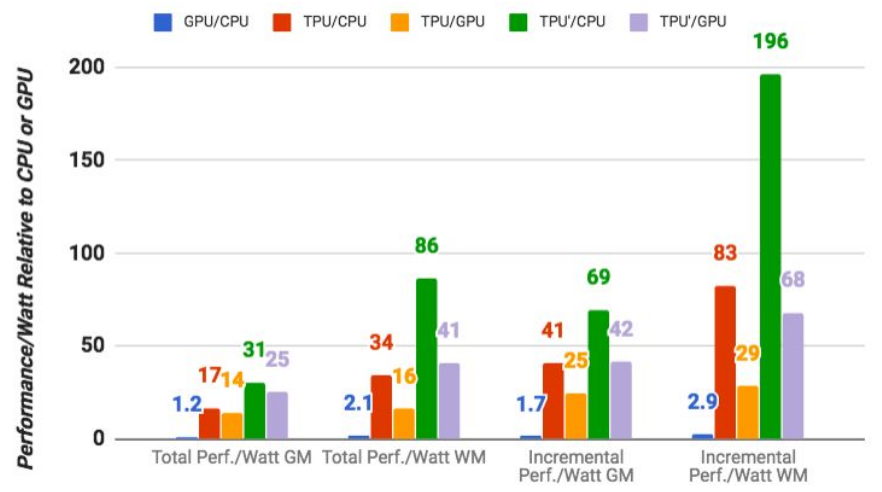
\includegraphics[width=\textwidth]{TPU_Relative_Performance.png}
  \caption{TPU performance, relative to CPU and GPU, the total performance includes server power costs. GM and WM are geometric and weighted means respectively \cite{Joup17}}
  \label{TPU_Relative_Performance}
\end{figure}

Other than the power efficiency the total processing power of a TPU is also far higher
than a GPU or CPU in figure \ref{TPU_Performance} where it can be seen that the pure
power of a TPU far outscales a CPU/GPU in most cases.

\begin{figure}
  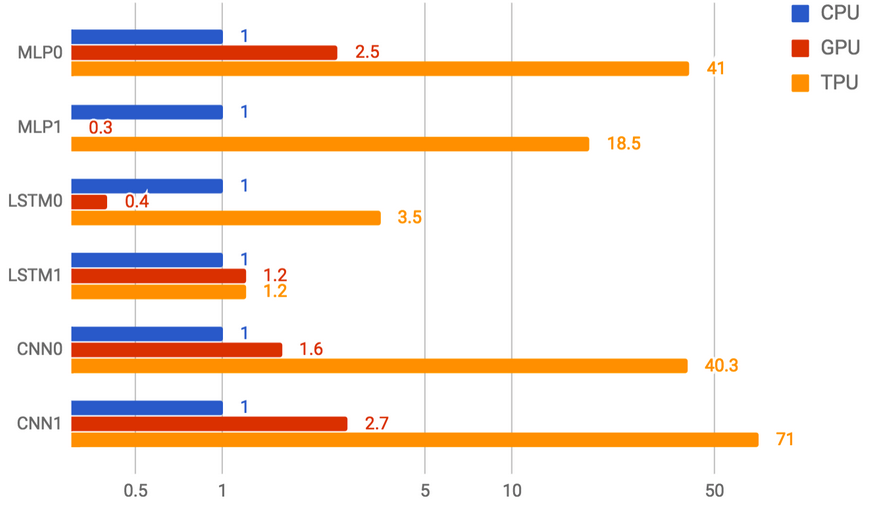
\includegraphics[width=\textwidth]{TPU_Performance.png}
  \caption{TPU performance on 6 common machine learning tasks\cite{Sato17}}
  \label{TPU_Performance}
\end{figure}


\paragraph{Computer architectures}
Other than using ASICs in order to increase the amount of work a computer can do
a different architecture can also be used that is deisgned to increase the amount
of useable cores on a computer massively. Such an architecture exists in the form
of the Epiphany architecture. The Epiphany architecture is a Multiple Instruction,
Multiple Data (MIMD) architecture that uses an array of processors, that all use the
same memory to speed up execution of floating point operations\cite{Olof16}.

The newest chip that Adapteva have managed to produce is the Epihpany V, which uses
1024 cores on a single chip\cite{Olof16}. Although the power consumption of their newest chip
is not yet public information, they have released numbers boasting a power usage of
only 2 watt on their Epiphany IV chip\cite{Adap}.

Using multiple processors to process one set of data is not a new idea in computer
Science, for this purpose MPI was developed to simplify the distribution of work,
usually over a cluster of workers. The same framework can also be adapted to the
Epiphany chips as was demonstrated by Richie et al. in their paper. They found that
the RISC chips were able to perform extremely fast matrix operations until their on board
memory was filled\cite{Rich15}. in figure \ref{Epiphany_MPI} it can be seen that performance increases
until the matrix no longer fits in memory.

\begin{figure}
  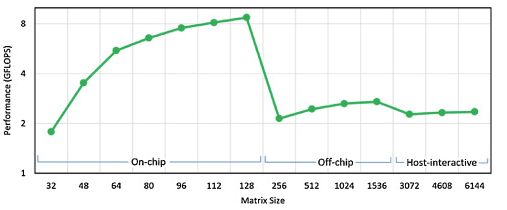
\includegraphics[width=\textwidth]{Epiphany_MPI.png}
  \caption{Epiphany chip performance with different matrix sizes\cite{Rich15}.}
  \label{Epiphany_MPI}
\end{figure}

\paragraph{Future relevance}
As can be seen with the examples above there are many different ways in which the
processing power needed for machine learning can be create. With both focusing
on power efficiency as well as computational power. However it must be noted,
that due to the benefits of space and power supply offered by a distributed system
all alternative solutions, work a lot better than a normal computer when not distributed
yet they all have the ability to be used together in a distributed setting without
loosing much if any in the form of performance. This makes them a good choice for
future applications, as they can use the benefits of both the improved hardware
and the distributed frameworks.
